\documentclass{beamer}
\usepackage[utf8]{inputenc}
\usepackage{babel}[spanish]

\usetheme{Madrid}
\usecolortheme{whale}


% Información de la página del título
\title{Introducción a \LaTeX}
\subtitle{Preparando documentos de alto nivel}
\author{ECEL Research Group}
\date{Abril 2021}

\begin{document}
\begin{frame}
 \maketitle   
\end{frame}
\begin{frame}{¿Qué es \LaTeX \ y por qué aprender a usarlo?}
\begin{itemize}
\item Es una herramienta para la preparación de documentos
\item Contiene facilidades que otros programas no tienen
\item \textit{What you see is what you get} vs. \textit{What you see is what you mean}
\item Utilizado para la creación de artículos científicos, libros, presentaciones, etc. 
\item Documentos de alto nivel, con formatos consistentes y complicados
\end{itemize}
\end{frame}
\begin{frame}{Nuestros objetivos}
 \tableofcontents
\end{frame}
\section{Breve historia}
\begin{frame}{Breve historia de \LaTeX}
\begin{minipage}[c]{0.55\textwidth}
 \begin{itemize}
     \item Creado por Leslie Lamport en 1984, cuando trabajaba en el SRI, como una herramienta para utilizar \TeX \ y escribir matemáticas avanzadas
   \item \TeX \  fue diseñado por Donald Knuth en 1978; un sistema de tipografía de alto nivel
     \item Para usar \LaTeX, se necesita una distribución \TeX  \ así como un programa que tenga los macros cargados
     \item La última versión es \LaTeXe, que reemplazó a \LaTeX \ 2.09
      \end{itemize}
     \end{minipage}
     \hfill
     \begin{minipage}[c]{0.4\textwidth}
     \centering
      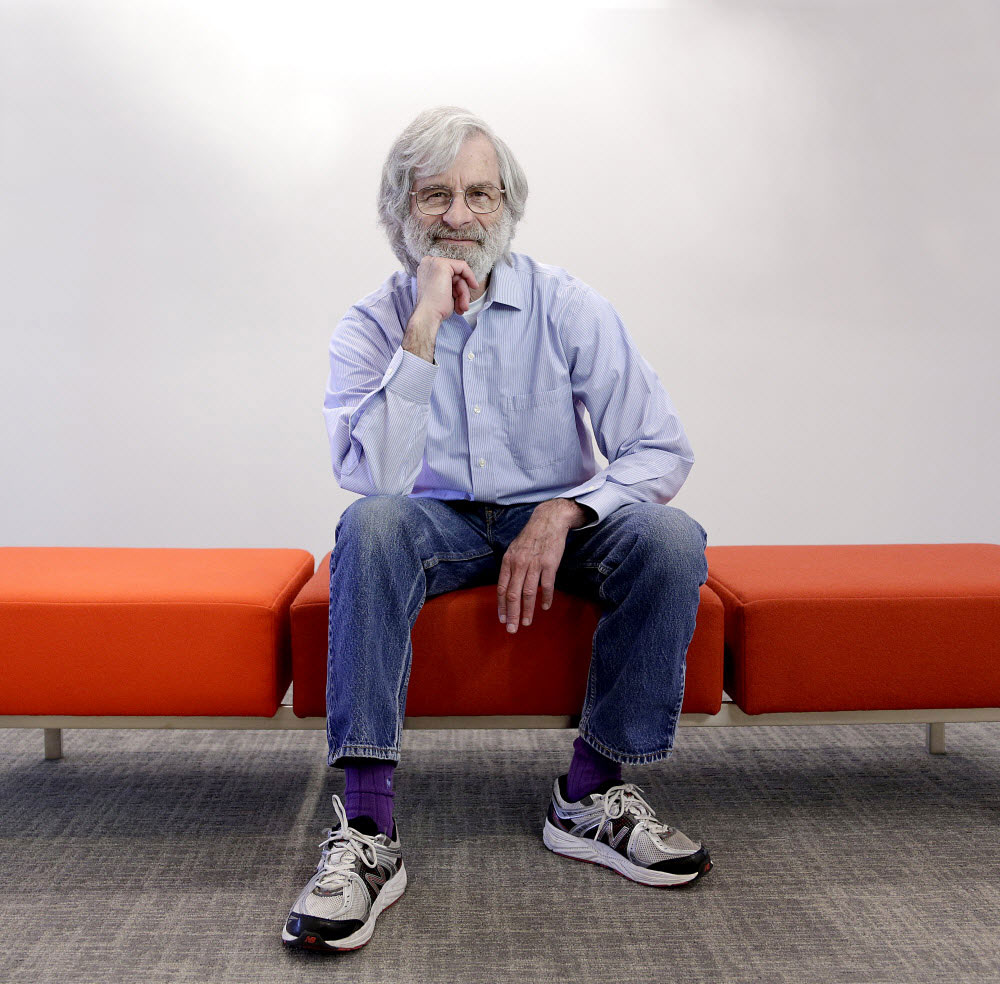
\includegraphics[scale=0.1]{fotos/lamport.jpg}
      \vspace{1cm}
      
           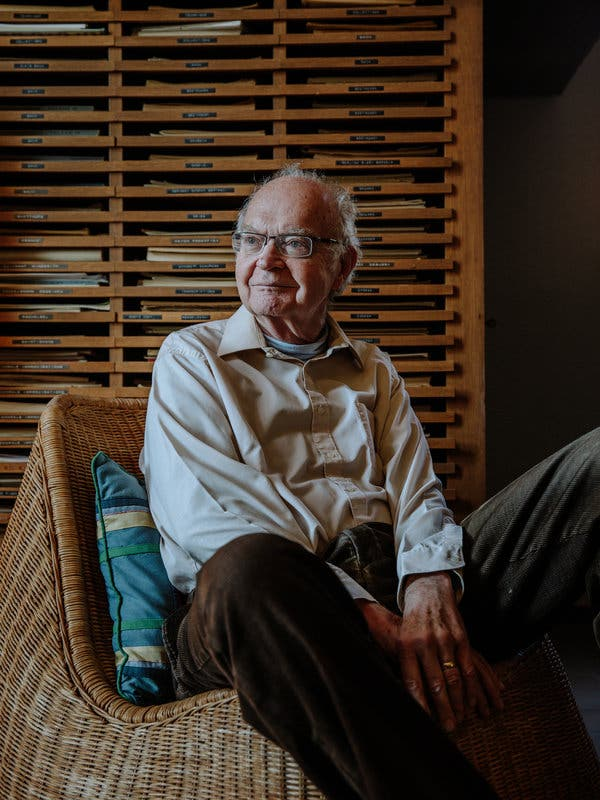
\includegraphics[scale=0.1]{fotos/knuth.jpg}
      \end{minipage}
\end{frame}
\section{Preliminares}
\begin{frame}{Localizando los caracteres más importantes}
    \begin{itemize}
        \item Para invocar comandos, \textit{backslash}: \textbackslash
             \item Para señalar que estas ingresando inputs a un comando, llaves: \{ \ \}
             \item Para hacer comentarios al script, porcentaje: \%
             \item Para dar argumentos opcionales a comandos, corchetes: [ \ ]
             \item Posiblemente es necesario cambiar el idioma o el \textit{layout} del teclado para hacer coincidir los caracteres
        \item Para la creación y manipulación de tablas: \&  
         \end{itemize}
         \centering
         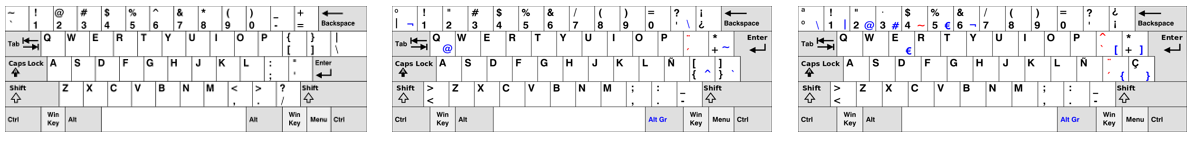
\includegraphics[scale=0.35]{fotos/teclados.png}
 \end{frame}
 \begin{frame}{Uso de \LaTeX \ en un computador}
\begin{itemize}
    \item Una distribución \TeX \ instalada
    \begin{itemize}
        \item Mik\TeX \ para Windows
        \item Mac\TeX \ para Mac
 \end{itemize}
   \item Un editor de \LaTeX \ para escribir los scripts
    \begin{itemize}
        \item \TeX maker
        \item Sublime Text 3
    \end{itemize}
     \item Un editor de \LaTeX \ online: Overleaf
     \begin{itemize}
         \item No necesita ninguna preinstalación
         \item Simple manejo de archivos del documento
         \item Un editor con facilidades excelentes
         \item Colaboración en tiempo real
         \item Requiere internet 
         \item Tiene límites como software gratuito
     \end{itemize}
  \end{itemize}
 \end{frame}
\section{Empezando un documento}
\begin{frame}{Preámbulo}
\begin{itemize}
    \item Aquí se especifican configuraciones para todo el documento, macros y paquetes
    \item Clases de documentos más comunes: 
    \begin{itemize}
        \item \texttt{article}
        \item \texttt{book}
        \item  \texttt{presentation}
        \item \texttt{report}
        \item \texttt{beamer}
        \end{itemize}
\item Los comentarios se deben escribir comenzando con un signo de porcentaje (\%)
\item Los comandos se invocan normalmente con un \textit{backslash}, parámetros obligatorios con llaves y parámetros opcionales con corchetes
\end{itemize}
\end{frame}
\begin{frame}{Comenzando a escribir}
\begin{itemize}
    \item Algunos parámetros default para un documento \texttt{article}:
    \begin{itemize}
        \item Tipo de letra tamaño 10, en libro es 11
        \item Orientación vertical
        \item 1 columna para el texto
    \end{itemize}
\item Para comenzar la segunda parte del archivo \LaTeX:
\texttt{\textbackslash begin\{document\}}
\item Todos los ambientes deben cerrarse con su respectivo \texttt{\textbackslash end\{\}}
\item El texto principal del documento está dentro del ambiente \texttt{document}
\item Lo mínimo que necesita \LaTeX \ para construir un documento es la clase de archivo y la ubicación del texto del documento en el script
\item Saltos de línea se deben hacer con doble \textit{backslash}: \textbackslash \textbackslash
\item Se deben utilizar comandos para los caracteres especiales
\end{itemize}
\end{frame}
\begin{frame}{Paquetes}
\begin{itemize}
    \item Adiciones a \LaTeX, nuevos comandos 
    \item Hace más simple algunos procesos que con \LaTeX\ base son complicados
    \item Paquetes fundamentales son \textsf{inputenc} con la opción \texttt{utf8} y \textsf{babel} con la opción de español (\texttt{spanish})
    \item Otros paquetes básicos son: 
    \begin{itemize}
        \item \textsf{geometry}; márgenes
        \item \textsf{setspace}; interlineado
        \item \textsf{lipsum}; \textit{dummy text}
            \end{itemize}
    
 \end{itemize}
    \end{frame}
    \section{Manejo de Texto}
    \begin{frame}{Estructura}
    \begin{itemize}
        \item Es convención utilizar estructura para ordenar el documento
        \item Es la base para crear tablas de contenido
        \item Diferentes subniveles para crear secciones
        \item La tabla de contenidos se genera automáticamente con \texttt{\textbackslash tableofcontents}
        \item Cuando existen cambios en la numeración, las tablas se actualizan solas
        \item Es posible editar la forma en la que aparecen los títulos
        \begin{itemize}
            \item Mediante la configuración de \textsf{babel} se cambia los predeterminados de todo el documento (para el idioma utilizado diferente a inglés)
        \end{itemize}
            \end{itemize}
    \end{frame}
    \begin{frame}{Portada}
     \begin{itemize}
         \item Como una alternativa al común \texttt{\textbackslash maketitle}
         \item Crea una página sin ningún formato (número o pie de página, encabezado si se ha hecho)
         \item Aquí se puede utilizar los comandos de tamaño de letra y formato para crear una portada
         \item Los ambientes de alineado especiales son claves para una buena portada
         \item Mediante \texttt{\textbackslash vspace} se puede espaciar con perfecta exactitud cada título en la portada
         \item Se puede seguir un formato específico de un trabajo dado por autoridades
     \end{itemize}
    \end{frame}
    \section{Manejo de matemáticas}
    \begin{frame}{Modo matemático}
    \begin{itemize}
    \item Utilizando símbolos especiales o la creación de un ambiente, se avisa a \LaTeX\  que estamos escribiendo matemáticas
    \item Las capacidades tipográficas son muy avanzadas y se puede escribir de lo más simple a expresiones ultra complejas
    \begin{block}{Ejemplo 1: Función Objetivo de la estimación MCO}
    El estimador de Mínimos Cuadrados Ordinarios para un modelo de regresión múltiple (para dos regresores) minimiza la expresión
    $$\displaystyle{\sum_{i=1}^{n} \left( y_i -\hat{\beta}_0-\hat{\beta}_1 x_{i1}-\hat{\beta}_2 x_{i2}\right)^2  }$$
    \end{block}
        \end{itemize}
    \end{frame}
 \begin{frame}{Modo matemático}
 \begin{itemize}

     \item Utilizar Word para este tipo de expresiones puede ser rápido e intuitivo para expresiones relativamente simples
     \item Sin embargo, para expresiones largas, o automatizar muchas expresiones  se vuelve poco eficiente
     \item Alinear las ecuaciones entre ellas es prácticamente imposible, y puede generarse un problema, como movimientos en imágenes
    \begin{block}{Ejemplo 2: Ecuaciones simultáneas para la minimización MCO}
    \tiny
    \begin{align*}
    \dfrac{\partial G}{\partial \hat{\beta_0}}&= \dfrac{\partial}{\partial \hat{\beta_0}}\left[ \sum_{i=1}^n \left(y_i-\hat{\beta_0}-\hat{\beta}_1x_i- \hat{\beta_2} z_i\right)^2 \right]= \sum_{i=1}^n\left[ \dfrac{\partial}{\partial\hat{\beta}_0} \left(y_i-\hat{\beta_0}-\hat{\beta}_1x_i- \hat{\beta_2} z_i \right)^2\right]=0\\
\dfrac{\partial G}{\partial \hat{\beta_1}}&=
       \dfrac{\partial}{\partial \hat{\beta_1}} \left[ \sum_{i=1}^n \left(y_i-\hat{\beta_0}-\hat{\beta}_1x_i- \hat{\beta_2} z_i\right)^2\right]=\sum_{i=1}^n\left[ \dfrac{\partial}{\partial\hat{\beta}_1} \left(y_i-\hat{\beta_0}-\hat{\beta}_1x_i- \hat{\beta_2} z_i \right)^2\right]=0\\
          \dfrac{\partial G}{\partial \hat{\beta_2}}&= \dfrac{\partial}{\partial \hat{\beta_2}} \left[ \sum_{i=1}^n \left( y_i-\hat{\beta_0}-\hat{\beta}_1x_i- \hat{\beta_2} z_i\right) ^2 \right]=\sum_{i=1}^n\left[ \dfrac{\partial}{\partial\hat{\beta}_2} \left(y_i-\hat{\beta_0}-\hat{\beta}_1x_i- \hat{\beta_2} z_i \right)^2\right]=0
    \end{align*}
    \end{block}
     \end{itemize}
 \end{frame}
 \begin{frame}{Modo matemático}
 \begin{itemize}
     \item El modo matemático, señalado por \$ \$ es la forma más directa de escribir matemáticas
     \item Automáticamente pone en un tipo de cursiva al texto, ignora espacios y permite comandos especiales
     \item Necesitaremos ubicar en nuestro teclado los siguientes caracteres: 
     \begin{itemize}
     \item Signo de dólar: \$
         \item Acento circunflejo (sombrerito): \^{}
         \item Guión bajo: \_
         \item ``Et'' (Ampersand) : \&
     \end{itemize}
 \end{itemize}
 \end{frame}
 \begin{frame}{Manejo Avanzado de Matemáticas}
 \begin{itemize}
     \item Mediante el uso de ambientes, se puede obviar los signos de dólar
     \item Se puede numerar y hacer \textit{cross-reference} a las ecuaciones, aplica también a tablas e imágenes
     \item La notación más avanzada suele tener problemas de visualización, normalmente se arregla con \texttt{\textbackslash displaystyle}
     \item La alineación se hace mediante el operador ``\&'', en ambientes que lo permitan\textbf{}
     \item Matrices funcionan de la misma manera que el ambiente \texttt{tabular}
     \item Se puede utilizar otro software para facilitar la utilización de matemáticas, pero no es infalible
\begin{itemize}
    \item Codecogs
    \item Mathpix Snip
\end{itemize}
 \end{itemize}
     
 \end{frame}
 \section{Gráficos}
 \begin{frame}{El paquete \textsf{graphicx}}
 \begin{itemize}
     \item Permite la utilización de imágenes en el directorio del script
     \item Para Overleaf, se debe subir las fotos al proyecto online
     \item Se maneja el tamaño de la imagen con parámetros opcionales
    \item El ambiente \texttt{figure} permite el posicionamiento de la imagen dentro del documento
    \item El paquete \textsf{float} permite una opción especial de posicionamiento
     \end{itemize}
 
 \end{frame}
\begin{frame}{Los paquetes \textsf{tikz} y \textsf{pgfplots}}
\begin{itemize}
    \item Para hacer gráficos directamente en \LaTeX \, como alternativa a usar imágenes
    \item El paquete \textsf{tikz} es la base de la construcción de gráficos, pero usarlo por sí solo puede ser algo complicado
    \item Utiliza una sintaxis diferente a la de \LaTeX\ común, usa puntos, paréntesis, comas, etc. 
    \item El paquete \textsf{pgfplots} trabaja a partir de \textsf{tikz}, es más directo
    \item Se puede graficar funciones, a partir de coordenadas, y leyendo archivos 
\end{itemize}
    \end{frame}
\section{Beamer}
\begin{frame}{Beamer}
\begin{itemize}
    \item Una clase de documento \LaTeX \ con opciones especiales para hacer presentaciones con diapositivas
    \item Hay otras formas, pero es la más simple de usar
    \item Se basa en \textit{frames}, que no necesariamente es igual a diapositivas de PowerPoint
    \item Un \textit{frame} puede tener diferentes ``diapositivas''
    \item Se maneja en base a temas (estilos) y colores de los mismos
    \item Tiene desventajas en el uso de animación, se hace en base al avance de diapositivas (no funciona como video)
\end{itemize}
\end{frame}
\section{Interfaz Overleaf}
\begin{frame}{Más sobre Overleaf}
\begin{itemize}
    \item Se puede hacer documentos colaborativos, mediante links
    \item Cuenta con un control de versiones y un chat entre colaboradores
    \item Se pueden descargar y subir los archivos \TeX\ para utilizarlos offline
     \item Se pueden hacer proyectos multi-archivo mediante el paquete \textsf{subfiles}
    \item Se construye un archivo principal, con un preámbulo que llama a todos los paquetes que se usan en todos los archivos
    \item Los otros archivos tienen una clase de documento especial, y también compilan por sí solos
    \item El \textit{subfile} usa el preámbulo del documento principal
\end{itemize}
\end{frame}
\section{Manejo de Bibliografías}
\begin{frame}{El paquete \textsf{biblatex}}
    \begin{itemize}
        \item Una alternativa a \textsf{natbib} o \textsf{bibtex}
        \item Utiliza un archivo externo, que puede ser generado desde una página web de citación o desde programas como Citavi, Mendeley, Zotero
        \item Con un ``índice'', se puede llamar a la fuente al documento y citarla con varios comandos del paquete 
        \begin{itemize}
            \item \texttt{\textbackslash parencite}
            \item \texttt{\textbackslash textcite}
        \end{itemize}
        \item Admite diferentes estilos:
        \begin{itemize}
            \item APA
            \item MLA
            \item Chicago
            \item Harvard
        \end{itemize}
    \end{itemize}
\end{frame}
\section{Integrando con otros programas}
\begin{frame}{Integración con Microsoft Word}
\begin{itemize}
    \item Algunos documentos de Word pueden requerir matemáticas avanzadas y no podemos pasarlos a \LaTeX:
    \begin{itemize}
        \item Tablas que se actualizan con Excel
        \item Se necesitan comentarios de alguien que no usa \LaTeX
        \item Formatos obligatorios para algunos trabajos
    \end{itemize}
    \item Se puede utilizar el editor de ecuaciones, pero hemos visto que no es eficiente
    \item En lugar de ello, podemos escribir código de \LaTeX \ base, con una opción especial en Word
    \item  No es demasiado avanzado, porque no podemos usar paquetes
    \end{itemize}
\end{frame}
\begin{frame}{Integración con R/Rstudio}
    \begin{itemize}
        \item El análisis estadístico avanzado normalmente requiere escribir un reporte en algún procesador de texto
        \item Puede ser complicado exportar los resultados de ese análisis al documento
        \item Con Rstudio, se puede simplificar el proceso con el paquete \texttt{stargazer}
        \item Es la opción más simple y rápida; produce resultados de alto nivel para diferentes elementos de R
        \item Existen herramientes más avanzadas, pero requieren más conocimiento de Rstudio
        \begin{itemize}
            \item \textsf{knitr}
            \item \textsf{sweave}
        \end{itemize}
    \end{itemize}
\end{frame}
\begin{frame}{Integración con Stata}
\begin{itemize}
    \item Se puede exportar a Excel las tablas que se generan mediante comandos de Stata
    \item Se selecciona los resultados deseados, click derecho y copiar tabla
    \item Eso se pega directamente a Excel, y luego se puede utilizar un \textit{table generator}
    \item Para las tablas de regresiones, se utiliza el paquete  \texttt{outreg2}
    \item Instalar en Stata mediante \texttt{ssc install outreg2}
    \item Realizar la regresión e inmediatamente poner \texttt{outreg2 using filename, append tex}
    \item Se puede exportar como Excel o también como archivo \TeX
\end{itemize}
\end{frame}
\begin{frame}{Debugging}
\begin{itemize}
\item \textit{Typos} son el error más común, por ende compilar constantemente es la mejor prevención para esos errores
    \item Tener proyectos \textit{multi-file} suele limitar las posibles localizaciones de los errores en documentos largos
    \item La definición incorrecta de ambientes también es un error común, pero Overleaf casi elimina esa posibilidad con su predictor
    \item Los errores más difíciles de corregir son cuando \LaTeX\ entiende algo diferente a lo que pretendíamos (no es exactamente un error)
    \item Pegar el log de errores en Google o formular/buscar una pregunta \TeX \ Exchange es la mejor manera de arreglarlos
    \item Los errores gramaticales/ortográficos pueden pasar desapercibidos, siempre pedir a alguien ser tu \textit{proofreader}
\end{itemize}
\end{frame}
\begin{frame}
\centering
 
\includegraphics[scale=0.5]{fotos/star-wars-training-grad.jpg}
\end{frame}

\end{document}
